%*******10********20********30********40********50********60********70********80
\DeclareFixedFont{\ttb}{T1}{txtt}{bx}{n}{12} % for bold
\DeclareFixedFont{\ttm}{T1}{txtt}{m}{n}{12}  % for normal
\definecolor{deepblue}{rgb}{0,0,0.5}
\definecolor{deepred}{rgb}{0.6,0,0}
\definecolor{deepgreen}{rgb}{0,0.5,0}

% Python style for highlighting
\lstset{
	backgroundcolor = \color{Ivory},
    language=Python,
    basicstyle=\footnotesize,
    otherkeywords={self},             
    keywordstyle=\footnotesize\color{deepblue},
    emph={__init__},          
    emphstyle=\footnotesize\color{deepred},    
    stringstyle=\color{deepgreen},
    frame=single,                         
    showstringspaces=false  ,
    breaklines=true,
    numbers=left,
    numberstyle=\footnotesize,
    tabsize=3,
    breakatwhitespace=false
}



% For all chapters, use the newdefined chap{} instead of chapter{}
% This will make the text at the top-left of the page be the same as the chapter

\chap{Approach and Design}
\section{Development Flow}
\vspace{-5mm}
\textbf{I Part: Data collection and validation}
\vspace{-5mm}
\begin{itemize}
 \setlength{\itemsep}{-5pt}
 \item Collect as many useful data as possible.
 \item Create a structured dataset that contains the collected data.
 \item Let the new data structure be accessable, available and readable.
 \item Let the data structure be an appropriate input to the analysis system used during the study.
\end{itemize}


\textbf{II Part: Systems implementation}
\vspace{-5mm}
\begin{itemize}
 \setlength{\itemsep}{-5pt}
 \item Analysis and displaying system implementation and results collection..
 \item Informations extraction.
 \item Prediction system implementation and results collection.
\end{itemize}


\textbf{III Part: Result, Discussion and Conclusions }
\vspace{-5mm}
\begin{itemize}
 \setlength{\itemsep}{-5pt}
 \item Results:
 \item Discussion:
 \item Conclusions:
\end{itemize}


\textbf{IV Part: Full code Implementation }

\newpage

------> I PART
During this phase the most important thing is to gather as much data as possible. The data have to be of course related with the current area of interest and they should be considered somehow useful for asnwering the initial questions of the study.\\
At the same time they should be as much reliable as possible since they are indispensable for the next phases and in particular for the final results and conclusions.\\
The data’s reliability mainly depends by which source they are coming from.\\
Then you should elaborate the data that you collected in order to:

------> II PART
This phase of the work will investigate about different ways for understanding and extracting information from the data.
For instance, the data will be displayed on different kind of graphics in order to increase their readable. Further more, several coefficients will be calculated and reported, always to allow the informations extraction from the data.
During this phase the main purpose is to predict some kind of useful data about the current dataset. To reach this goal, is first of all indispensable to choose a prediction system to implement. \\
Once the prediction system has been implemented, it's time to apply it on the current data and try to get as much evidences as possible.

------> III PART
The results part contains

The purpose of the discussion is to interpret and describe the significance of this thesis results. Further more, has to be reported a critical evaluation about the work done and explain any kind of limitations found during the procedure.
The conclusion part has to contains a summarize about what was done in this thesis, and then figure out some other extra ideas, implementations or recommendations to future work about this thesis.\\
\begin{figure}[h]
    \makebox[\textwidth][c]{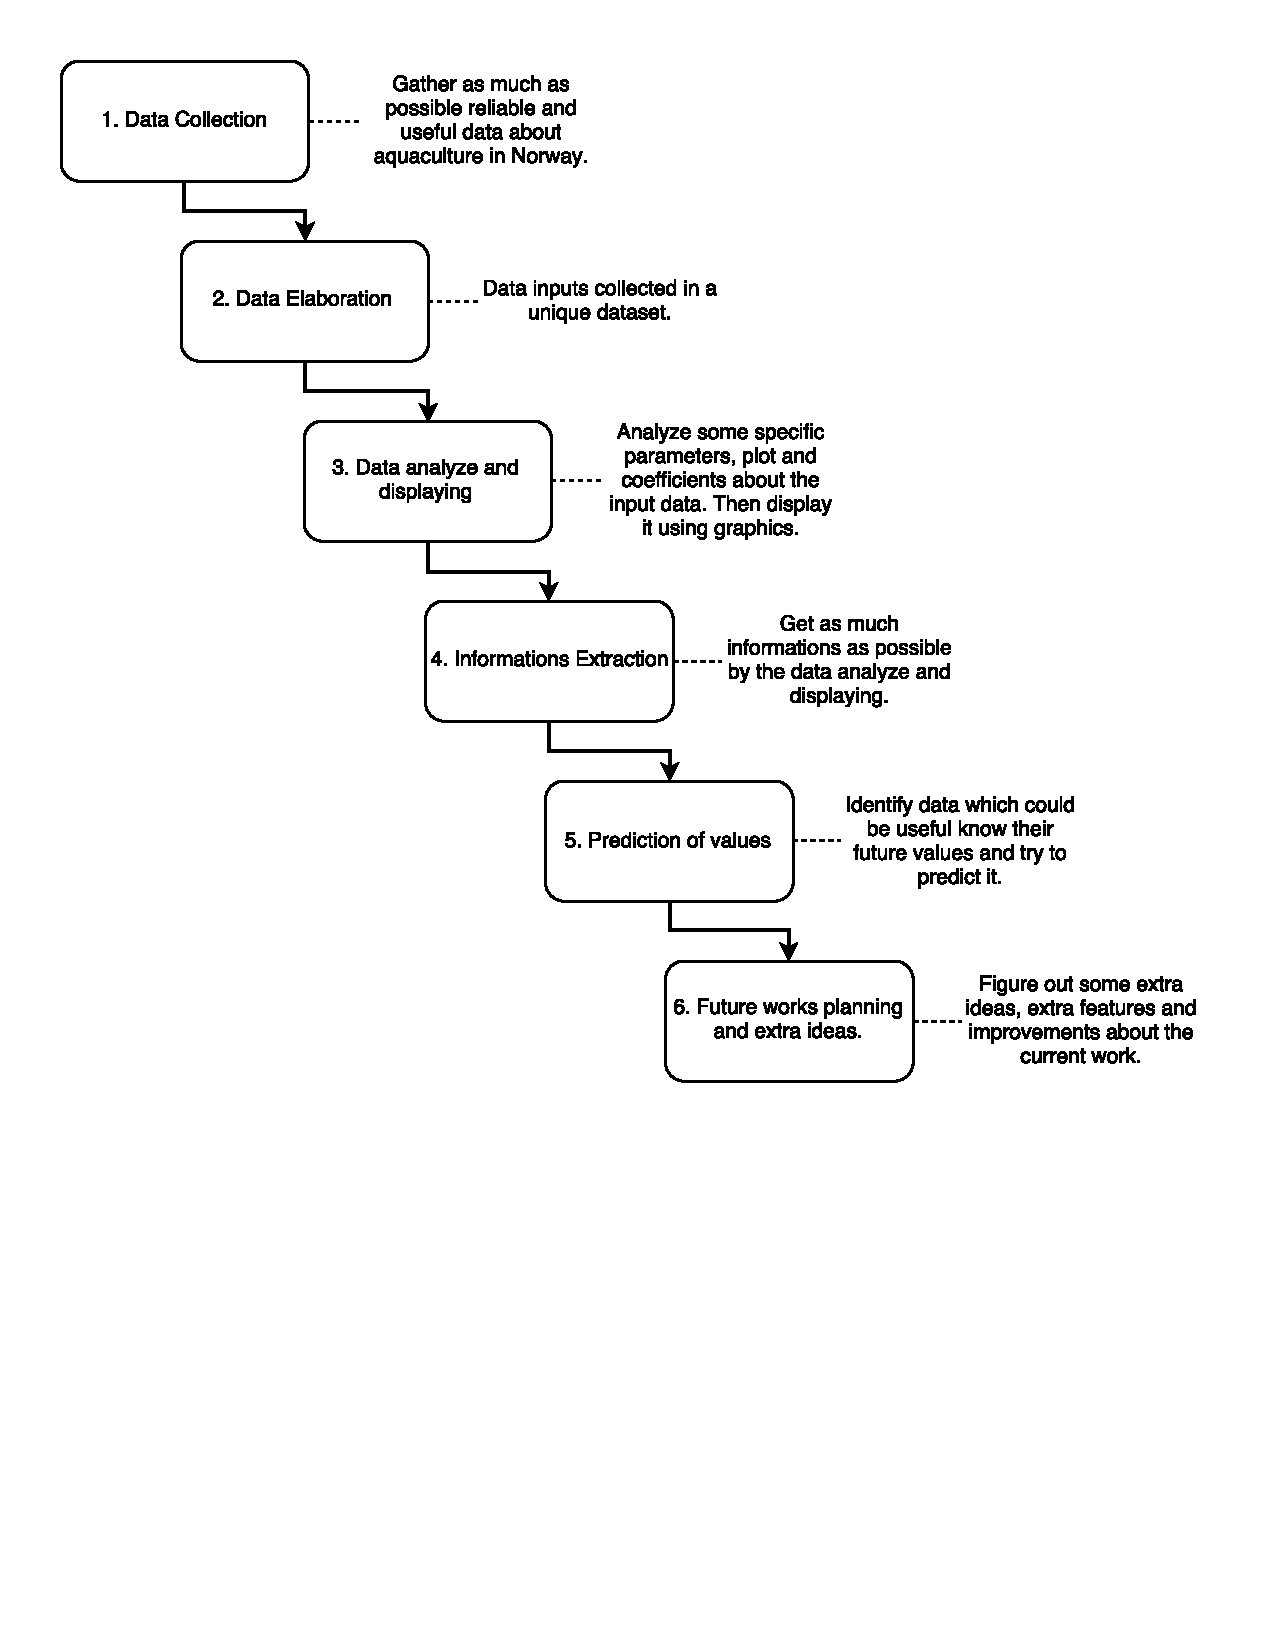
\includegraphics[width=1.1\textwidth,natwidth=761,natheight=681]{Files/DevelopmentFlow.pdf}}
    \caption[Plan flow chart]{Plan flow chart}
    \label{fig: Development_Flow}
\end{figure}


\section{Important recommendation}
Before start to read the implementation procedure about this work, it's important to know that is possible to find the system's full implementation on Github.\\
I \textbf{strongly recommend} to check it out and download the following repository. It allows to test the system and better understand how it is structured and how it works.\\
Further more, it's possible to find inside the same repository all the needed datasets and a "Manual" wich contains the instructions about how to use it.

The Github repository is:\\
\url{https://github.com/Sprea22/Python_Systems}

The direct Zip file download is:\\
\url{https://codeload.github.com/Sprea22/Python_Systems/zip/master}

